\chapter{Overview}

\section{Project Aims}
\subsection{Improving the performance of dynamic languages when executing data-driven tasks}
Dynamic, interpreted languages are commonly celebrated for their increased succinctness over static, compiled languages. Often, they greatly reduce the amount of code that is necessary to perform common tasks. However, they continue to be overshadowed by the throughput resultant from heavily optimised compilation of static languages, particularly for performance-intensive procedures. A typical performance divergence is shown in Figure~\ref{fig:ruby_vs_c}.

\begin{figure}[h]
  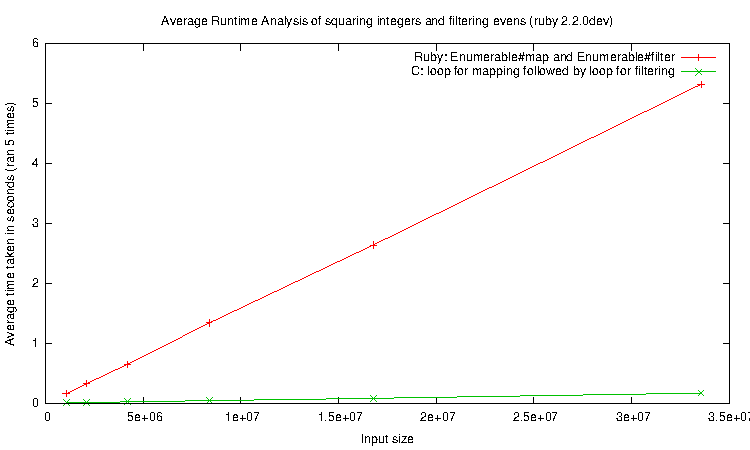
\includegraphics[width=\textwidth]{./figures/ruby_vs_c.pdf}
  \caption{Graph demonstrating the significant difference in performance when operating on large datasets in C and Ruby.}
  \label{fig:ruby_vs_c}
\end{figure}

RubiCL aims to investigate and mitigate any decreased performance experienced when using the Ruby language for data processing. By producing a more efficient implementation of computational tasks, users will be able to tackle larger scale problems without needing to learn new toolchains.

\paragraph*{Indicators of success}
Progress towards this goal can be evaluated by comparing the performance of data-driven computation tasks in Ruby, with and without the library's contributions, to that of functionality provided by native extensions written in static languages. Further success can be measured by investigating whether increased magnitude computation now terminates within reasonable time, due to the project's contributions.

\subsection{Facilitating a larger scale of experimentation in a REPL environment by non-expert users}

An interactive environment, such as a \ac{REPL}, is commonly useful for rapid prototyping. It allows online processing of data without the need to produce all of the required code upfront, as shown in Listing~\ref{lst:repl}. \acp{REPL} are absent from many languages. In supported languages, they allow the user to continuously query data and return intermediate results. Often, a quick turnaround between idea and response leads to more questions. This can enable an investigational attitude to computer programming.

\begin{lstlisting}[
  language=Ruby,
  label=lst:repl,
  caption=A basic example of using a REPL environment for data analysis.
]
dataset_1.mean
# =!> NoMethodError: undefined method `mean' for Array

module Enumerable
  define_method(:mean) { map(&:to_f).inject(&:+) / size }
end
#=> :mean

dataset_1.mean
#=> 23.6

dataset_2.mean
#=> 23.2
\end{lstlisting}

By widening the scope of problems that can be evaluated within a \ac{REPL}, RubiCL shall enable a larger scale of investigation. Analysis of particularly large datasets is currently unavailable to novice users, due to the amount of computation required.

\paragraph*{Indicators of success}
The completed library should be presented to novice analysts, users with mathematical insight but insignificant programming prowess. If they are able to easily answer queries about large datasets, the system's design will be judged as successful. As with the previous goal's evaluation, response time within a \ac{REPL} environment will be examined.

\subsection{Exploring the extensibility of the Ruby programming language}
Ruby has served as a suitable foundation for many \acp{DSL}, including build tools\cite{rake} and web frameworks\cite{sinatra}.

The language has open classes, whereby the structure of object classes can always be altered at run-time, even after definition ends. It also permits a variety of meta-programming techniques, allowing complicated code to appear misleadingly simple at the surface.

\begin{lstlisting}[
  language=Ruby,
  label=lst:sinatra,
  caption=The Sinatra DSL for simple web programming hides complexity when writing basic web services.
]
require 'sinatra'

get '/hi' do
  "Hello World!"
end
\end{lstlisting}

Objects in Ruby are often regarded as \emph{duck-typed}. This means that the system should care only about how an object behaves \textemdash{} ``If it looks like a duck, swims like a duck, and quacks like a duck, then it probably is a duck.''\cite{ducktest}

Since function invocation uses a \emph{method-sending} approach, the underlying implementation can be altered significantly as long as an expected dialog is presented to the run-time.

This project demonstrates integrating drastically different processing techniques into the language's run-time. It achieves this without greatly affecting the code that a user must write in order to use them.

\paragraph*{Indicators of success}
The integration will be successful if the interface for processing data remains consistent. Parallelism should be implicit and not requiring direction from the programmer. Again, user testing will evaluate this.

\subsection{Effective code generation and reuse on the OpenCL platform}
\ac{OpenCL} can provide high throughput computation, often utilised by bespoke systems such as cryptographic hashers and video encoders. However, there is a significant amount of configuration and set-up code associated with each parallel tasks performed. Code reuse is difficult to achieve on the \ac{OpenCL} platform due to the specificity of kernel execution.

Without techniques for reuse, advances made by one parallel project may not be applicable to others. In this case, programmers writing parallel systems must implement all subtasks from the bottom up when constructing the full solution. As it is hard to incorporate the partial solutions of others, barriers to entry are further increased.

This project undertaken will attempt to recycle the partial solutions of primitives as much as possible. This allows investigation into how much reuse is possible, given an ideal system with a single author.

With greater code reuse, optimisations of a given subtask will improve all primitives utilising the component. This directs experimentation when searching for performance improvements.

\paragraph*{Indicators of success}
Unfortunately, code reuse is often best measured subjectively. Yet, the developer's opinion when reflecting on the development experience may provide useful insight. If code reuse techniques facilitate the development of this particular \ac{OpenCL} project, it is likely that they may be beneficial to developers elsewhere.

\subsection{Applicability to a variety of platforms, avoiding over-tailoring for a specific machine}
The project should be packaged in a manner that facilitates installation onto a new, supported, system. In addition, it should achieve performance enhancement without having to be adjusted significantly by the user.

As a result, no assumptions about the specific hardware present can be made, apart from full \ac{OpenCL} support. This will allow the project to support a range of current and future compute-devices.

\paragraph*{Indicators of success}
Deployment of the system to new hardware will be attempted, after the development phase has concluded. If the system remains performant and the deployment procedure does not require change, this is evidence of sufficient hardware agnosticism.


\section{Leveraged Software Components}
The project will provide functionality to users through utilisation of two previous bodies of software: The \ac{OpenCL} library and the Ruby programming language.

\subsection{OpenCL}
The project requires interaction with heterogeneous processing devices present within a user's system.
It achieves this via the hardware vendor's implementation of the \ac{OpenCL} library.

\ac{OpenCL} is an open framework for executing tasks, described by C99-syntax \emph{kernels}, on a variety of devices.
Suitable targets include a range of heterogeneous devices such as multi-core \acp{CPU}, \acp{APU}, and \ac{GPU} from the majority of commodity hardware vendors.

The Khronos Group maintains and frequently updates the \ac{OpenCL} standard\cite{khronos}.
Participating vendors include \ac{AMD}, Apple, Intel, and NVIDIA \textemdash{} although the quality and accessibility of implementations varies greatly.

A stated goal of the \ac{OpenCL} project is to ``allow cross-platform parallel programming''.
The underlying processing devices present on a system are abstracted, allowing code to be written without explicit knowledge of target architectures.
This theoretically enables developers to write applications for a person system and then later scale execution to a massively parallel workstation, without significant code modification.

\begin{figure}[h]
\begin{center}
	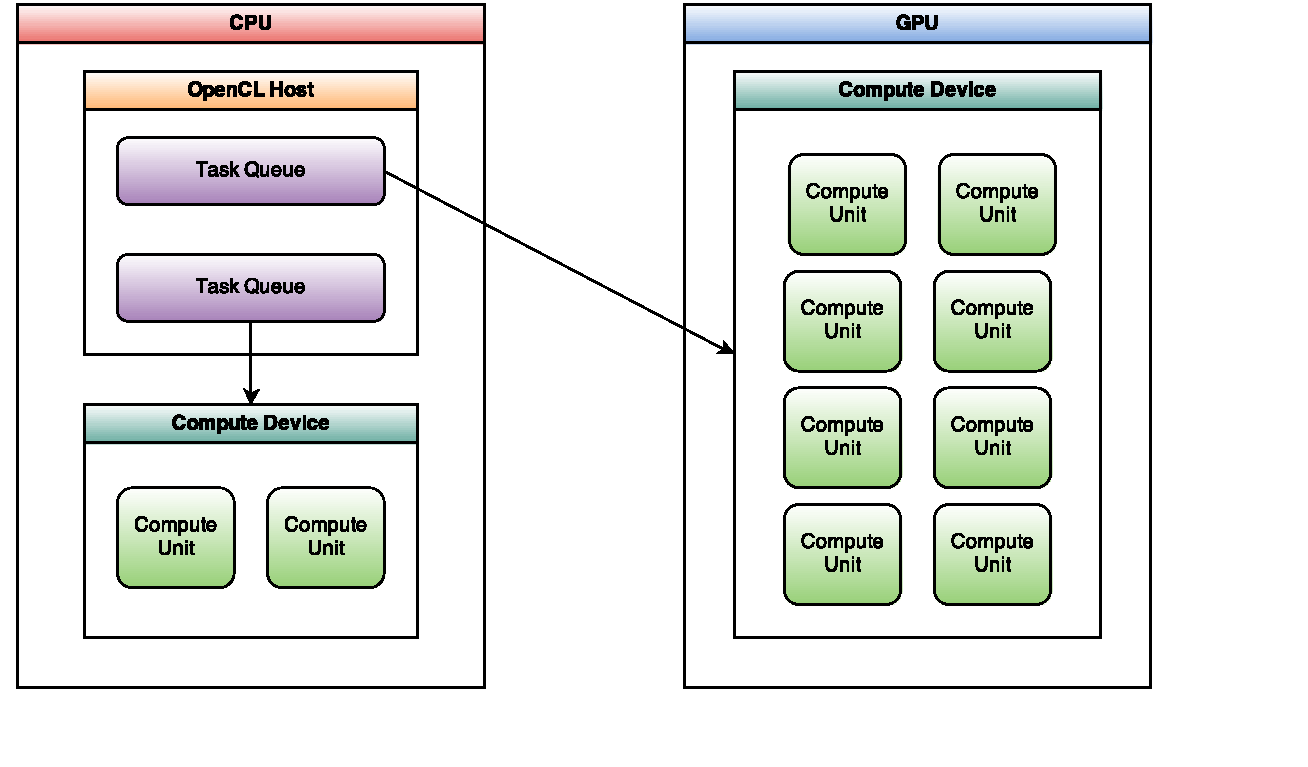
\includegraphics[width=4.8in]{./figures/OpenCLModel}
	\captionof{figure}{The OpenCL architecture model.}
	\label{fig:ocl_model}
\end{center}
\end{figure}

\paragraph*{Architecture model}
As Figure~\ref{fig:ocl_model} illustrates, the architecture model presented by \ac{OpenCL} is as follows:

\begin{description}
\item[Host device] The system's \ac{CPU}. It interacts with an execution environment, responsible for discovering and selecting compute devices present on the system. The host device initialises one or more \emph{contexts}, whereby any devices within a single context have access to shared task and memory buffers.

\item[Compute devices] The system's available processing devices, capable of scheduling \ac{OpenCL} kernel work-groups. Before enumerating compute devices, the available \emph{platforms} must be discovered by the runtime. Usually, there is a platform presented for each unique \ac{OpenCL} supporting vendor with hardware installed. Devices are then retrieved on a per-platform bases, either filtered by type (\ac{CPU}/\ac{GPU}) or not.

\item[Compute Units] Discrete units of hardware present within a processing devices, capable of scheduling and executing \ac{OpenCL} kernel instances.
Kernel execution occurs across internal \emph{processing units}, such as \acp{ALU}.
\end{description}

\begin{figure}[h]
	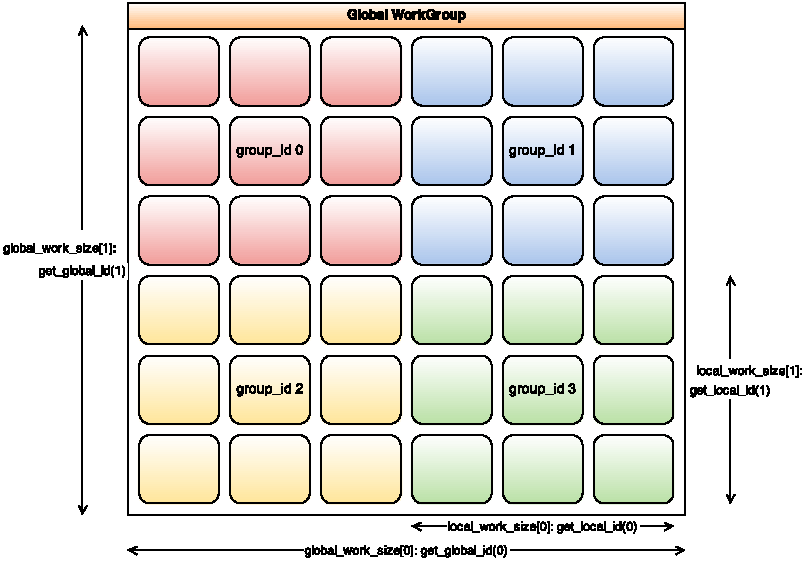
\includegraphics[width=4.8in]{./figures/workgroups}
	\captionof{figure}{The OpenCL execution model.}
	\label{fig:ocl_ex_model}
\end{figure}

\paragraph*{Execution Model}
\ac{OpenCL} has a simple execution model, allowing both \emph{coarse-grained} and \emph{fine-grained} parallelism. Programmers write parallel code from the reference frame of a single kernel execution. Each instance orients itself only via access to its \emph{local} and \emph{global} \verb|id|, expanded on shortly. Larger calculations are a direct result of cooperating kernel instances. 

Kernel instances, scheduled for execution on compute devices, as referred to as \emph{work-items}.

The \ac{OpenCL} standard calls a collection of work-items a \emph{work-group}. Work-groups are the unit of work dispatched to a device. The number of work-items within a group that a device should schedule is set by the programmer, providing the \verb|global_work_size| parameter. Each kernel invocation is enumerated with a global \verb|id|. 

In addition to flat enumeration, the computation can benefit from the abstraction of work \emph{dimensions}. For example, a calculation over $100$ elements can represented as a 2-dimensional $10 \times 10$ calculation. When utilising dimensional abstraction, access to either unique global \verb|id| or $x, y$ offsets is available.

Higher dimensions are available for further structuring of tasks. It is clear that the spatial abstraction provided when there is a topological significant within the processed data. In these circumstances, the \verb|local_work_size| parameter provides further benefits.

When \verb|local_work_size| is specified, again possibly with dimensionality, the work-items are additionally divided into subgroups. Memory allocation can use the \verb|__local| qualifier. In this case, data will reside in higher-bandwidth buffers that can only be synchronised between members of the same local work-group. With the addition of this second, local tier of memory, the \ac{OpenCL} model hints at how efficient kernels should be constructed. Being aware of the positioning of data and its dependencies is key to developing efficient kernels, free of memory-synchronisation bottlenecks.

Much of the project's implementation effort concerning \ac{OpenCL} will be mapping data required by common algorithms to efficient arrangements within device memory. This mirrors \ac{OpenCL} development in general.
The fact that this task is so laborious is a reason why heterogeneous parallel programming is still under-utilised in the wild.

\paragraph*{Comparison with CUDA}
\ac{OpenCL} is not the only computation framework choice when interacting with \ac{GPGPU} devices. As mentioned earlier, a competing technology is NVIDIA's \ac{CUDA}.

During the planning phase, RubiCL considered both choices. Ultimately, the decision was made to use \ac{OpenCL} over \ac{CUDA} for several major reasons:

\begin{description}
  \item[Multiple vendor support]
    \ac{CUDA} is not an open standard. Its parallelism framework is only available on NVIDIA hardware. Using a library supported only by a single vendor to provide the project's hardware interfacing would lead to far fewer systems being able to benefit from accelerated processing.

  \item[CPU and GPGU execution]
    By using \ac{OpenCL}, RubiCL will be able to execute kernels on both \ac{CPU} and \ac{GPGPU} devices. This contrasts the \ac{GPGPU}-only focus of \ac{CUDA}.
    This greatly increases development convenience. Development can occur on a mobile laptop, functionally tested with its \ac{CPU}. Afterwards, the library will be transferred to desktop workstations for performance testing on a variety of hardware.

    In addition, this opens up the possibility of attempting code execution on both devices concurrently. This will investigate whether complete system-wide utilisation is beneficial for a single computation.
  \end{description}

  \paragraph*{Disadvantages of choosing \ac{OpenCL}}
  There are several downsides to using \ac{OpenCL} instead of \ac{CUDA}. The programming model is generally agreed to be less developer friendly. This is perhaps due to the need to include far more abstraction over the range of target devices. In addition, due to the need for compatibility with several device families, \ac{OpenCL} can be less performant out-of-the-box than \ac{CUDA}. Advanced knowledge of how to tweak device-specific parameters to avoid execution bottlenecks can help avoid this.

  \paragraph*{Current state of OpenCL implementations}
  A final major disadvantage of \ac{OpenCL} at the moment, is the current quality of some vendor implementations. All vendors advertise themselves as being \ac{OpenCL}-compatible when marketing their hardware. However, in reality it is harder than advertised to achieve a working system.

  For example, NVIDIA, have made no attempt to hide the fact that they would much rather everybody used \ac{CUDA} instead. They are so slow at releasing libraries that they are a full version of the \ac{OpenCL} specification behind other vendors at the time of writing this report. Features that are supported also perform much worse than expected.

  Intel are up-to-date with library implementations but only have non-Windows support if you have purchased non-consumer grade \emph{Xeon} processors.

  Hopefully these issues will be rectified if \ac{OpenCL} continues to gain tracking in future. As a short term response, the RubyCL project has been implemented on well-supported hardware only: An Apple Macbook Air containing a Intel Haswell processor, and a desktop system containing an \ac{AMD} \ac{CPU} and \ac{GPU}.

  Apple and \ac{AMD} both have high-quality \ac{OpenCL} $1.2$ libraries and seem to be the two companies most invested in increased \ac{OpenCL} uptake. Apple have recently started encouraging desktop software developer to schedule suitable tasks on the \ac{GPU} via OS X's \ac{GCD}.


\subsection{Ruby}
\paragraph*{Language features}
Ruby\cite{rubylang} is an interpreted, dynamic language, embracing a variety of programming paradigms. It contains many features designed to increase its extensibility via meta-programming.

Execution centres around the creation of objects, every class inherits from at least \verb|BasicObject|. Function invocation is triggered by sending the target object a \emph{message}.

Upon receipt of a message, it is handled by the lowest level of an objects inheritance-hierarchy \textemdash{} the composed chain of class and module extensions that are mixed-into the object instance. A level will either respond to the message or, if unable to, propagate the request further up the chain.

A common meta-programming technique is to redefine how a module within the hierarchy responds when a method definition is missing. Instead of simply passing the message to the next level, it can inspect the name and arguments of the function, or its own state, and give a response. This cancels further progression of the request.

\begin{comment}
\begin{lstlisting}[
  language=Ruby,
  label=lst:methmiss,
  caption=A toy example where an object responds to a missing method instead of propagating the message.
]
class HungryHippo
  def eat
    puts "Nom nom nom!"
  end

  def method_missing(meth, *args, &block)
    if /eat/.match meth.to_s
      puts "Eat? ok then."
      eat
    else
      super
    end
  end
end

hippo = HungryHippo.new
hippo.eat
hippo.dont_eat
# >> Nom nom nom!
# >> Eat? ok then.
# >> Nom nom nom!
\end{lstlisting}
\end{comment}

This flexibility is often used (or abused) to reduce the amount of boilerplate code written.

In addition to dynamically responding to received methods, objects are often substituted for objects of another class that have subtly different behavior. This will be successful as long as they respond the same method calls. Therefore, it is common practice to consider only the interface presented by interacting objects and not their individual types.

The benefit of this \emph{duck-testing} is that the same series of of method requests, present in a line of code, can cause very different patterns of computation. If the response of a single link in the chain is altered, the programmer would be unaware, and unconcerned, as long as the expected pipeline result is returned.

This technique of redirecting computation will be explored by the RubiCL library. It allows a decoupling of the programmer's requests and the underlying, massively-parallel implementation.

\paragraph*{Native extensions}
The latest versions of the Ruby language make it simple to produce native extensions. Functionality is provided by C shared-objects that interact with the underlying \ac{RubyVM}.

\begin{lstlisting}[
  language=C,
  label=lst:native_ext1,
  caption=The C code defining a module with the ability to perform native actions.
]
#include "ruby.h"
#include "something_native.h"

/* All Ruby objects are of type VALUE and must be unboxed */
/* Every method takes self as an explicit argument */
VALUE
methodSomethingNative(VALUE self, VALUE int_param_object) {
    int param  = FIX2INT(int_param_object);
    int result = doSomethingNative(param);

    return INT2FIX(result);
}

void /* module_example is name defined in Makefile */
Init_module_example() {
    VALUE ModuleEx = rb_define_module("ModuleExample");
    /* Visibility, Module, Name, Method, Arg count. */
    rb_define_private_method(
        ModuleEx, "something_native",
        methodSomethingNative, 1);
}
\end{lstlisting}

Adding native methods is as simple as performing the heavy-lifting as one would in a pure C application. The \verb|ruby.h| library then allows the programmer to create a Ruby module or class with mappings between method names and the underlying implementations.

\begin{lstlisting}[
  language=Ruby,
  label=lst:native_ext2,
  caption=A Ruby class utilising a native extension module.
]
require './module_example'

class NativeThing
  include ModuleExample

  def method_requiring_native
    something_native(1)
  end
end
\end{lstlisting}

The required complication of converting between Ruby objects and basic C types is handled via macros, defined for all sensible conversions.

Once an extension has been compiled, the shared-object file is \verb|require|d and the constructed object is available, no differently to a pure Ruby implementation. In the case of RubiCL, modules for particular concerns are provided and then mixed-into classes that require native functionality.

\paragraph*{Suitability as the project's target language}
The project decided to use Ruby as the target language as, alongside Python, it is often recommended to beginners for analytics and \emph{data-science}. This is perhaps due to the syntax being relatively straightforward and often self-documenting.

Unlike Python, Ruby's design is less opinionated about the \emph{principle of least surprise}, and therefore makes it much easier to drastically extend its capability while hiding complexity from unaware users. 

In addition, the need for constant method-hierarchy lookup has been blamed for its poor performance. The potential for dynamic redefinition of methods complicates caching and can heavily impact certain compute-intensive tasks. This makes Ruby a suitable target for a project aiming to offer an optimised library for such tasks.


\section{Project Progression}
\subsection{Timeline}
\paragraph*{Initial focus}
In the project's first year, most of the time was spent researching existing parallel frameworks. The project's initial goal was to present a \emph{MapReduce} runtime. Therefore, systems like \verb|Phoenix++|\cite{phoenix++} and \verb|StreamMR|\cite{streammr} were evaluated.

Part-way through the year, during prototyping, it became clear that there are several disadvantages to producing (yet-another) \emph{MapReduce} system:
\begin{itemize}
\item The runtime resource management is overkill on a singular, massively parallel machine. When isolated failure is unlikely, more lightweight processing paradigms can be used with greater efficiency.

\item Previous projects have hit issues caused by \ac{GPGPU} architecture. For example, tasks that emit tuples must be run twice: Once to count the number of tuples emitted, and again to actually produce the results. This is needed as \ac{OpenCL} kernels do not allow dynamic allocation of memory.

\item Since \ac{OpenCL} compute devices execute only kernels, there are just two options for task specification:

Firstly, users can specify tasks in \ac{OpenCL} kernel form. This is terrible for system usability. Products such as \emph{Hadoop} are successful due to features such as the \emph{streaming \ac{API}}, allowing code to be written in familiar languages when performing parallel tasks on tuple streams.

Secondly, the system could translate an existing language into \ac{OpenCL} kernels. This would allow users to stay within their comfort zone yet still utilise the parallel architecture of many modern systems. Unfortunately, this task is an enormous undertaking. Progress has made recently on generating \ac{CUDA} executables from LLVM \ac{IR}, yet similar breakthroughs for the \ac{OpenCL} platform are lacking.
\end{itemize}

\paragraph*{Moving away from MapReduce}
There are clear benefits of utilising familiar languages for orchestrating parallel tasks, such as significant increases in usability.
Yet, it is currently infeasible to translate the entirety of stated programs.
With this in mind, the decision was made  to lower the scope of direction, with the user stating only parallel subroutines and having \ac{OpenCL} dispatch of said subroutines automated.

At the close of the first year, a prototype system was produced that allowed a user to perform \verb|map| and \verb|filter| tasks.
Specification of tasks was provided by a string of C expressions that would be interpolated into stock kernels.
\begin{lstlisting}[
  language=Ruby,
  label=lst:project_prototype,
  caption=Example of prototype system workflow.
]
DataSet.create(
  name: :one_to_ten,
  type: :int,
  data: (1..10).to_a
)

FP::Map.create(
  name: :add_one,
  key: [:int, :i],
  function: 'i += 1;'
)

FP::Filter.create(
  name: :add_three_is_even,
  key: [:int, :i],
  function: 'i += 3;',
  test: 'i % 2 == 0'
)

DEVICE = OCLDevice::CPU.get

DEVICE
  .load(:one_to_ten)
  .fp_map(:add_one).fp_filter(:add_three_is_even)
  .output
\end{lstlisting}
This proof-of-concept demonstrated that performance gains were achievable by performing computation outside the confines of the \ac{RubyVM}.

However, evaluation of the prototype highlighted several flaws:
\begin{itemize}
    \item Using the library was incredibly verbose. Creating named objects to represent each state of computation meant that a line of pure Ruby code could spawn tens of lines of library code when converted to parallel execution.

    \item Lots of redundant parameters were required by the system. There is no reason for a \verb|map| task to specify it's input parameter type when the syntax can be checked by a compiler. The separate declaration and usage of element variables increased the potential for bugs, in addition to exposing implementation details to the user.

    \item A lack of task optimisation caused higher-than-necessary workloads. Two consecutive \verb|map| tasks would require two passes over the data instead of just one, as the intermediate result was produced.

    \item Code quality was poor. This was mainly due to the combination of venturing into a previously unexperienced programming paradigm, and organic growth of functionality during rapid prototyping.

    A prototype with successful functionality is used to discover the requirements of a system. It is then much easier to redesign a new system, one that is much more elegant yet achieves the same results.
\end{itemize}

\paragraph*{Learning from mistakes}
The system redesign at the start of the second year specifically targeted previously identified flaws:
\begin{itemize}
    \item First-class function support allows the library's usage to mirror standard higher-order function usage. Since anonymous function are used, this removes the verbosity of many named objects requiring creation.

    \item Some parameters are no-longer required, or inferred, due to a change in internal design. For example, anonymous functions document the input parameter throughout the calculation, so specifying this separately is unnecessary.

      Another example is subroutine type information. The computation pipeline can now keep track of the buffer type at a given point in execution and use this to guide kernel creation, instead of requiring user-submitted type definition.

    \item By deferring and combining tasks, as documented in the \emph{Design} chapter, unnecessary computation can be avoided.

    \item A redesigned architecture, alongside focusing on testing and ease-of-modification. This helps maintain the software quality of the replacement system, even as requirements shift.
\end{itemize}

\subsection{Difficulties}
Several unforeseen issues have slowed down progress in certain stages of the project's progression.

\paragraph*{Initial development system}
The target \ac{GPGPU} test-bed was originally a desktop system containing a NVIDIA \emph{GTX 670} \ac{GPU}. It also contained an Intel \emph{Haswell} \ac{APU}. Unfortunately, it became clear during the process of porting the codebase, initially developed solely on a MacBook, that the state of the required libraries was much worse than advertised.

Had the libraries for the system been available, the produced framework would allow task scheduling on either compute device within the \ac{APU}, or the \ac{GPGPU}.

The difficulties encountered were as follows:
\begin{itemize}
  \item Intel's \ac{OpenCL} implementation only allows access to the graphics-processing \ac{APU} co-processor under two conditions: If the operating system is Windows 7/8, or if the device is a Xeon processor. Xeon devices are not present in affordable desktop systems. The owned test-system did not support the required socket-style.

  \item Development in Windows was not possible due to the need to build several system components. The latest Ruby language snapshot and the extension modules necessary for the library to operate must be built, from source, during development. This process is still bug-ridden on non-*NIX systems.
\end{itemize}

Following these setbacks, the goal of utilising the \ac{APU}'s graphic subsystem in addition to the \ac{CPU} was abandoned. \emph{GNU/Linux} was installed on the desktop system. However, the situation was further hindered when it became clear that the capabilities of NVIDIA's \ac{OpenCL} implementation were vastly overstated. With no support for \ac{OpenCL} $1.2$ and suboptimal performance on $1.1$m the high-end \ac{GPU} present would not provide as much of a performance boost as initially anticipated.

\paragraph*{Replacement system}
In order to continue the project's goal of properly exploring the potential benefits of \ac{GPGPU} programming, the decision was made to purchase an `idea' hardware platform to continue development on.

The system, consisting of an \ac{AMD} \emph{FX-4130} CPU and an \ac{AMD} \emph{R7 260X} \ac{GPGPU}, was ordered and assembled after the initial problems were encountered. This caused a slight stall in development. However, it was estimated that with hardware utilising a single, \ac{AMD} \ac{OpenCL} implementation, productivity would be vastly increased. In fact, this was the case, enough so to make the delay worth experiencing.`

\section{Completed Work}
\subsection{Features}
\todo{Complete overview of what was done, brief but inclusive.}
